\documentclass[10pt]{article}

\usepackage[margin=0.7in]{geometry}
\usepackage{graphicx}
\usepackage{booktabs}
\usepackage{amsmath}
\usepackage{siunitx}
\usepackage{caption}
\usepackage{subcaption}
\usepackage{microtype}
\usepackage{enumitem}
\usepackage{hyperref}

\graphicspath{{figures/}}
\setlength{\parskip}{3pt}
\setlength{\parindent}{0pt}
\captionsetup{font=small, skip=4pt}

\title{\vspace{-3em}Predicting Remaining Soot Mass from a SiC--ZnO/LSCO DC Sensor:
A Feature--Ablation Study}
\author{}
\date{\vspace{-2.5em}}

\begin{document}
\maketitle
\vspace{-2em}

\textbf{Goal.}
Quantify how much of the remaining soot mass during a temperature--ramped
oxidation can be predicted from the SiC--ZnO/LSCO sensor's DC resistance alone,
and how much an additional (independently measured) temperature improves the
prediction. Although in DC mode the sensor's scalar resistance physically
aggregates several effects --- conventionally written
\(R_{\text{total}} = R_{T} + R_{\text{soot}} + R_{\text{config}} +
R_{\text{gas}} + R_{\text{else}}\) --- this study does \emph{not} attempt to
estimate those terms separately. The question we answer is the strictly
operational one: ``given $(R)$ or $(R,T)$ as inputs, how well can a regression
model recover the gravimetric soot mass?''.

\textbf{Data.}
Aligned from \texttt{12-02-2025 raw sensor data.xlsx}: Resistance (interpolated
from \texttt{TIME-sensor} onto the DC clock), Temperature (\texttt{Temp-DC}),
and ground--truth remaining mass (\texttt{Soot left-mg}, from the
\texttt{calculation} sheet). After dropping the post--reaction tail
(\texttt{Time-DC}~$>$~\SI{17500}{\second}, no further combustion), $n=379$
samples remain. A single random 50/50 split (\texttt{seed=0}; 189 train, 190
test) is applied identically to both feature sets. Train/test CSVs are
committed under \texttt{data/}.

\textbf{Models.}
Ten standard regressors, no per--model tuning.
\begin{itemize}[leftmargin=*, itemsep=0pt, topsep=2pt]
    \item \emph{Linear / Ridge / Lasso / ElasticNet} -- fit
          $\hat y = a_1 R + a_2 T + b$, differing only in how large
          coefficients are penalised. Cannot capture curvature.
    \item \emph{SVR (RBF kernel)} -- fits a smooth, locally adaptive surface in
          $(R,T)$ via Gaussian basis functions.
    \item \emph{$k$--Nearest Neighbours ($k=5$)} -- averages the soot mass of
          the 5 nearest training samples in scaled $(R,T)$ space; purely local.
    \item \emph{Decision Tree, Random Forest, Gradient Boosting,
          HistGradientBoosting} -- partition $(R,T)$ into rectangles and
          predict the mean target per partition. RF averages 500 trees;
          boosting fits trees sequentially to residuals.
\end{itemize}

\textbf{Pairwise correlations.}
Pearson measures linear, Spearman measures monotonic association.
Resistance--Temperature are strongly anti--correlated (semiconductor behaviour);
the resistance--mass map is monotonic but markedly non--linear (large Spearman,
smaller Pearson), so any resistance--only predictor must be non--linear to
exploit it.

\begin{center}\small
\begin{tabular}{lrr}
\toprule
Pair & Pearson $r$ & Spearman $\rho$ \\
\midrule
Resistance vs.\ Temperature   & $-0.799$ & $-0.966$ \\
Resistance vs.\ Soot mass     & $+0.599$ & $+0.932$ \\
Temperature vs.\ Soot mass    & $-0.929$ & $-0.966$ \\
\bottomrule
\end{tabular}
\end{center}

\textbf{Ablation results.}
With resistance only, the best non--linear model (Decision Tree) reaches
$R^{2}=0.804$, MAE~$=\SI{0.046}{\milli\gram}$. Linear models cap at
$R^{2}=0.352$, confirming the curved $R\!\to\!\text{mass}$ map. Adding
temperature collapses the prediction error by an order of magnitude across
every family: the best two--feature model (RBF--kernel SVR) reaches
$R^{2}=0.9997$, MAE~$=\SI{0.0025}{\milli\gram}$. Even the linear models jump
to $R^{2}=0.914$, mirroring the near--linear Temperature--mass relationship in
the correlation table.

\begin{table}[h]\centering\small
\caption{Test $R^{2}$ on the 190--sample random test set; $\Delta R^{2}$ is
the gain from adding temperature.}
\label{tab:r2}
\begin{tabular}{lrrr}
\toprule
Model & Resistance only & Resistance + Temperature & $\Delta R^{2}$ \\
\midrule
SVR (RBF)                    & $0.731$ & $0.9997$ & $+0.27$ \\
Gradient Boosting            & $0.659$ & $0.9996$ & $+0.34$ \\
KNN ($k=5$)                  & $0.769$ & $0.9996$ & $+0.23$ \\
Random Forest                & $0.717$ & $0.9995$ & $+0.28$ \\
HistGradientBoosting         & $0.784$ & $0.9994$ & $+0.22$ \\
Decision Tree                & $0.804$ & $0.9994$ & $+0.19$ \\
Linear / Ridge / Lasso / EN  & $0.352$ & $0.914$  & $+0.56$ \\
\bottomrule
\end{tabular}
\end{table}

\begin{figure}[h]
\centering
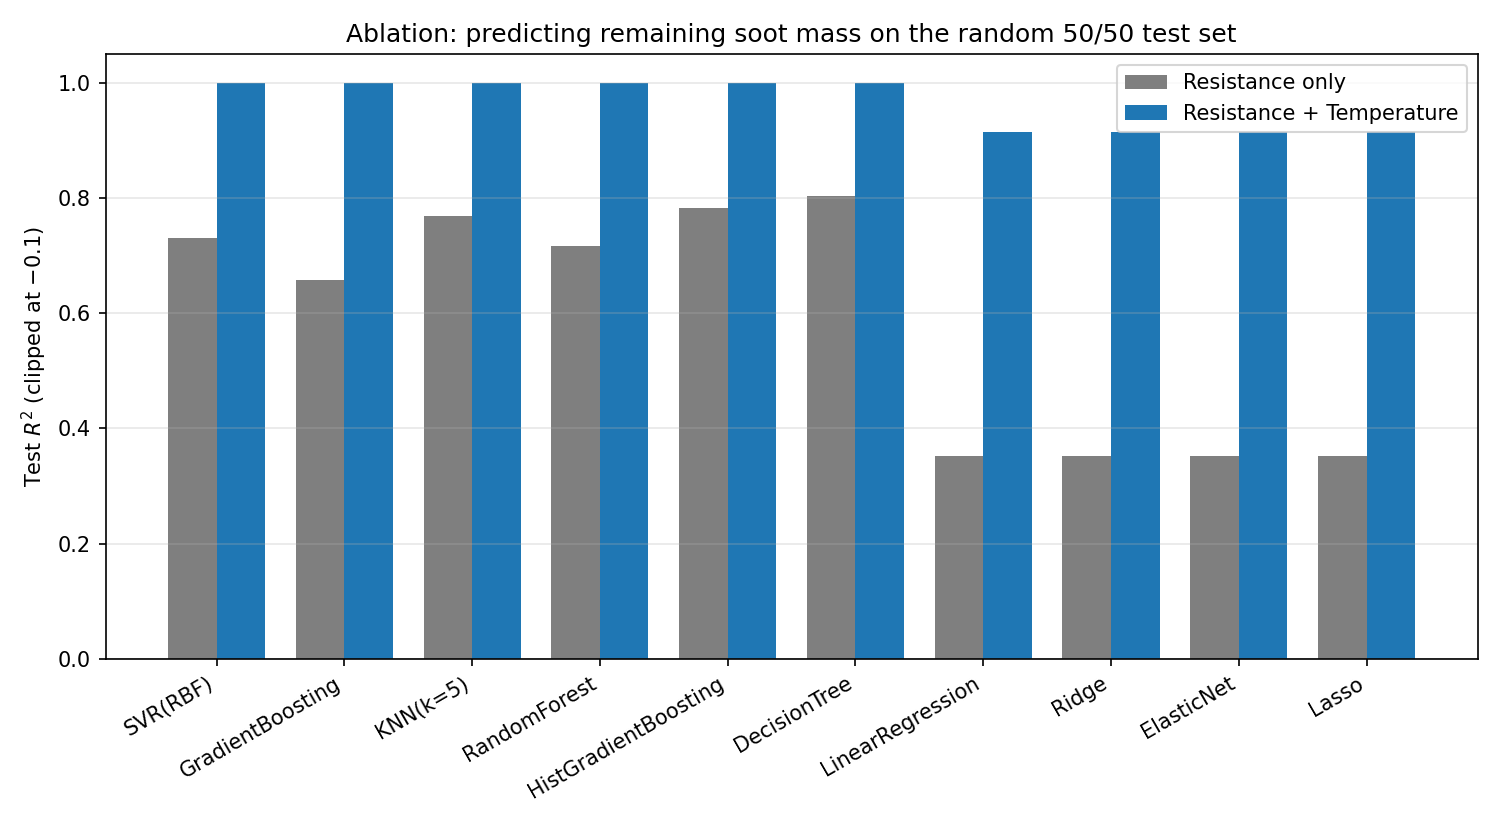
\includegraphics[width=0.72\textwidth]{ablation_r2.png}
\caption{Gray bars: each model trained on resistance only. Blue bars: same
model trained on resistance + temperature. Adding temperature improves every
model --- the six non--linear models climb from roughly $0.65$--$0.80$ to
nearly $1.0$, and the four linear models from $0.35$ to $0.91$.}
\label{fig:ablation}
\end{figure}

\textbf{Prediction quality, visualised.}
Fig.~\ref{fig:bestpred} contrasts the best model under each feature set on
the held--out test points, sorted by time. The resistance--only Decision Tree
captures the bulk descent of the soot mass but exhibits visible scatter and
piecewise--flat segments characteristic of a shallow tree fit to a single
non--linear input. The Resistance\,+\,Temperature SVR traces the measured
curve essentially exactly: the two lines are visually indistinguishable
across the entire test range.

\begin{figure}[h]
\centering
\begin{subfigure}[t]{0.49\textwidth}
    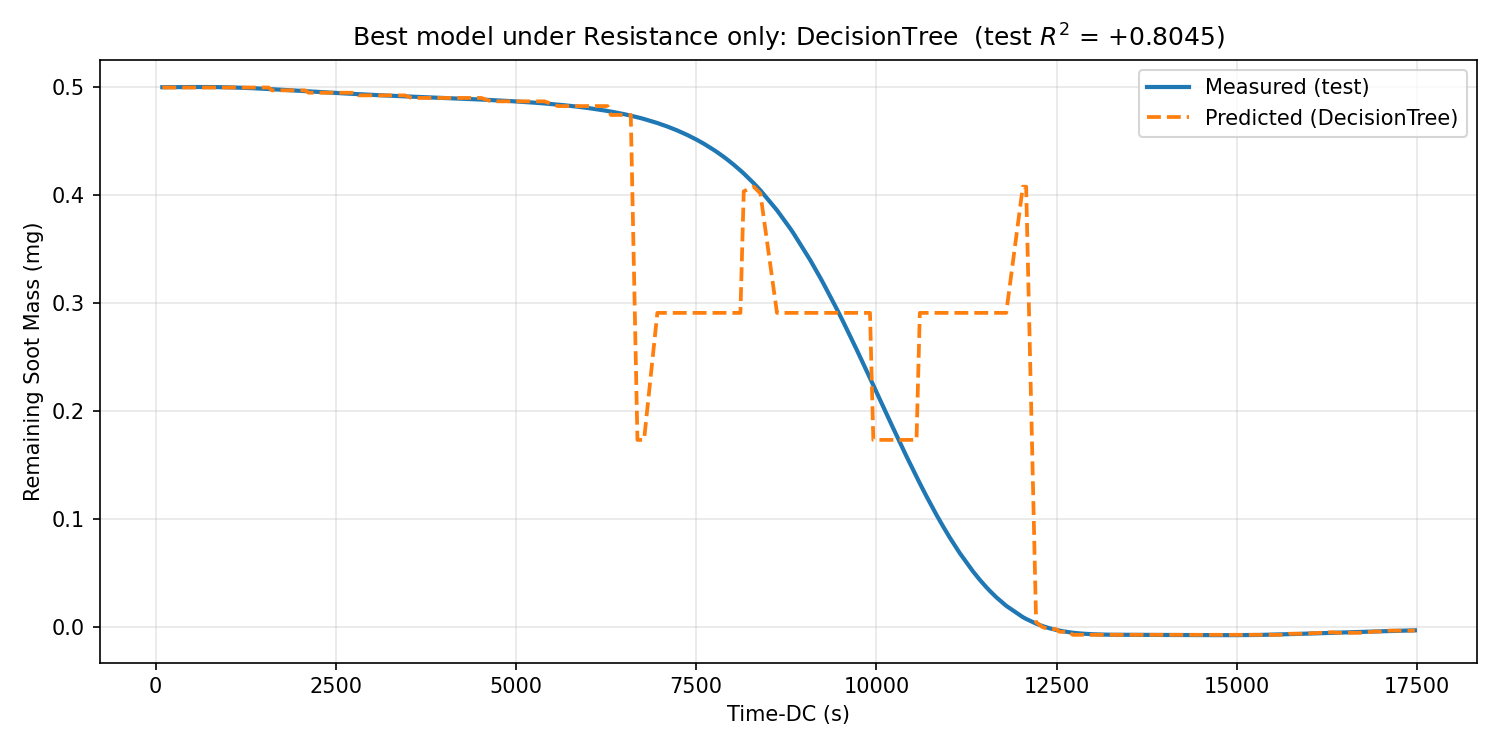
\includegraphics[width=\textwidth]{best_pred_resistance_only.png}
    \caption{Resistance only --- Decision Tree, $R^{2}=0.804$.}
\end{subfigure}\hfill
\begin{subfigure}[t]{0.49\textwidth}
    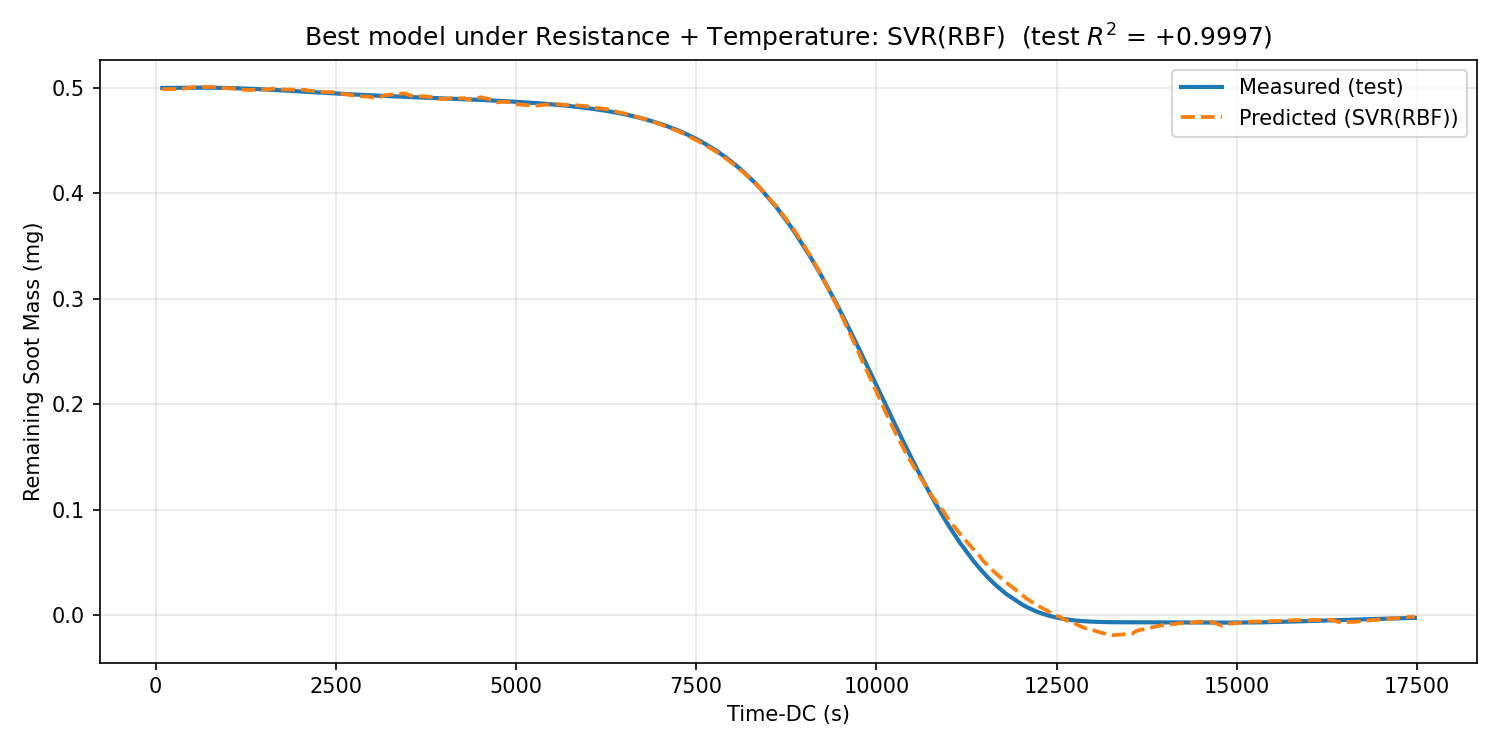
\includegraphics[width=\textwidth]{best_pred_resistance_temp.png}
    \caption{Resistance + Temperature --- SVR (RBF), $R^{2}=0.9997$.}
\end{subfigure}
\caption{True vs.\ predicted remaining soot mass on the test set, sorted by
time, for the best model under each feature set.}
\label{fig:bestpred}
\end{figure}

\textbf{Can we say how much of the prediction comes from temperature vs.\
resistance?} Not from this dataset. Because the experiment is a single
temperature ramp, resistance and temperature move in lockstep throughout
(their rank correlation is $-0.97$, see correlation table above). When two
inputs are this strongly co--ordered, the standard tools that try to split
credit between them --- feature--importance scores from a tree, coefficients
from a linear fit, partial--dependence plots --- can attribute the same
predictive power to either input depending on which model is used, and the
answer is therefore a modelling artefact rather than a physical
decomposition. What the ablation \emph{does} establish is qualitative and
robust: both inputs are required for the model to reach its best score
(resistance alone tops out at $R^{2}=0.80$; the linear models drop from
$0.91$ down to $0.35$ when temperature is removed), and together they
reproduce the entire mass trajectory. Cleanly separating the
temperature--driven and resistance--driven contributions to the prediction
would require an experiment in which soot loading is varied at fixed
temperature, so that resistance changes while temperature does not --- a
follow--up that is outside the scope of this report.

\textbf{Discussion.}

\emph{What the sensor can deliver today.}
With a thermocouple providing a temperature reading alongside the sensor, the
combined two--feature model predicts the remaining soot mass to within
${\sim}\SI{0.003}{\milli\gram}$ on the test set --- precise enough to use as a
quantitative mass tracker during an oxidation experiment, replacing or
augmenting a gravimetric measurement. With resistance alone (no independent
temperature reading), the best non--linear model still tracks the overall mass
trajectory ($R^{2}\!\approx\!0.80$, residuals ${\sim}\SI{0.05}{\milli\gram}$,
a few percent of the initial soot loading). That accuracy is sufficient for
qualitative monitoring tasks --- detecting that oxidation is occurring,
estimating when the burn--out completes, comparing the shapes of two
oxidation runs --- but not for absolute mass quantification.

\emph{Why the headline $R^{2}=\!0.9997$ is partly optimistic.}
The $379$ samples form a single, smooth oxidation curve, and we partitioned
them by random shuffle. As a result, almost every test point has a training
point recorded only ${\sim}\SI{30}{\second}$ earlier or later, with nearly
identical resistance, temperature, and soot mass. Flexible models (KNN,
Decision Tree, RBF--kernel SVR) exploit this by effectively
\emph{interpolating} between adjacent training samples --- a much easier task
than predicting on a genuinely new experimental run. The reported scores
should therefore be read as ``how well the model fills gaps in an
already--sampled trajectory'', not as a guarantee that the model would do
equally well on a future ramp run with a different rate, a fresh soot
deposit, or a different SiC--ZnO/LSCO device.

\emph{What would strengthen the conclusions.}
Three follow--up experiments would address the open questions raised by this
report. (i) Repeat the analysis with a chronological train/test split --- fit
on the early portion of the ramp, test on the late portion --- to verify the
model genuinely extrapolates across the oxidation phase rather than
interpolating within it. (ii) Collect multiple oxidation runs with different
temperature programmes (different ramp rates, or isothermal holds at
$\SI{450}{\celsius}$ as in the NO/O$_2$ pulse experiments in the PDF
appendix) and test whether a model fitted on one transfers to the others.
(iii) Run experiments in which soot loading is varied while temperature is
held fixed, which breaks the lockstep between $R$ and $T$ and is the only way
to attribute, separately and physically, how much of the sensor signal is
genuinely soot--driven rather than thermally--driven.

\textbf{Reproducibility.}
The single script \texttt{dc\_soot\_mass\_report.py} at the repository root
regenerates every CSV in \texttt{data/} and every PNG in \texttt{figures/}
from the raw spreadsheet (random seed \texttt{0}).

\end{document}
